The core concept was first presented for the one-dimensional 0-1 knapsack problem (KP),
leading to very successful KP algorithms.
The main idea is to reduce the original problem by only considering a set of
items for which it is hard to decide if they will occur or not in an optimal solution.
This set of items is named core.
The variables for all items outside the core are fixed to certain values.

The KP considers items $j = 1, \ldots, n$, associated profits $p_j$ and
associated weights $w_j$.
A subset of these items has to be selected and packed into a knapsack having capacity $c$.
The total profit of the items in the knapsack has to be maximized, while the
total weight is not allowed to exceed $c$.

If the items are sorted according to descreasing efficiency values
\begin{displaymath}
  e_j = \frac{p_j}{w_j},
\end{displaymath}
it is well known that the solution of the LP-relaxation consists in general of
three consecutive parts: The fisrt part contains variables set to $1$, the second
pare consists of at most on split item $s$, whose corresponding LP-values is
factional, and finally the remaining variables, which are always set to zero,
form the third part.
For most instance of KP (except those with a very special structure) the integer
optimial solution closely corresponds to this partitioning in the sense that it
contains most of the highly efficient items of the first part, some items with
medium efficiencies near the split item, and almost no items with low efficiencies
from the third part.
Items of medium efficiency constitute the so called core.

Balas and Zemel~\cite{balas1980algorithm} gave the following precise definition
of the core of a KP, based on the knowledge of an optimal integer solution $x^*$.
Assume that the items are sorted according to descreasing efficiencies and let
\begin{displaymath}
  a := \min\{ j | x_k^* = 0 |\}, \quad b := \max\{ j | x_j^* = 1 \}.
\end{displaymath}
The core is given by the items in the interval $C = \{a, \ldots, b\}$.
It is obvious that the split item is always part of the core.

The KP Core problem (KPC) is defined as
\begin{align*}
  \text{maximize} & \sum_{j \in C} p_j x_j  + \tilde{p}\\
  \text{subject to} & \sum_{j \in C} w_{j} x_j \leqslant c - \tilde{w}\\
  & x_j \in \{0, 1\}, \quad j \in C.
\end{align*}
with $\tilde{p} = \sum^{a-1}_{j=1} p_j$  and $\tilde{w} = \sum^{a-1}_{j=1} w_j$.
The solution of KPC would suffice to compute teh optimal solution of KP, which
however, has to be already partially known to determine $C$.
Nevertheless an approximate core $C = \{s-\delta, \ldots, s+\delta\}$,
of fixed size $|C| = 2\delta+1$ is considered for a heuristic reduction of the problem.

Figure~\ref{fig:kpcore} exemplifies the core of a hypothetical KP instance with
$13$ items.
The first row represents the efficiency value of each item and the second row
represents the value of each variable on the LP-relaxation optimal solution.
The items are sorted in descending order of efficiency value.
The last row illustrates the variable fixing after the defined core.
An asterisk indicates a free variable.

\begin{figure}[h]
  \centering
  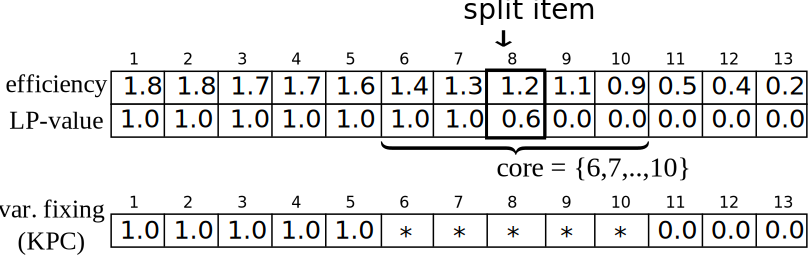
\includegraphics[scale=0.37]{imgs/kp_2}
  \caption{Example of core for a hypothetical KP instance with $n=13$ and core size of $5$ ($\delta = 2$).}
  \label{fig:kpcore}
\end{figure}

\subsection{The Core Concept for MKP}

The previous definition of the core for KP can be extended to MKP without major
difficulties, once an efficiency measure is defined for the MKP,
as addressed in \cite{puchinger2006core}.
Even though a proper efficiency measure for MKP is not obvious due the
multidimensional weight of the items.
A well accepted efficiency measure is discussed in Section~\ref{subsec:dual}.

Let $x^*$ be an optimal solution and assume that the items are sorted in
descending order after a given efficiency. Then let
\begin{displaymath}
  a = \min \{ j | x_j^* = 0 \}, \quad b = \max \{ j | x_j^* = 1 \}.
\end{displaymath}
The core is given by the items in the interval $C = \{ a, \ldots, b \}$,
and the multidimensional knapsack core problem (MKPC) defined as
\begin{align*}
  \text{maximize} & \sum_{j \in C} p_j x_j  + \tilde{p}\\
  \text{subject to} & \sum_{j \in C} w_{ij} x_j \leqslant c_i - \tilde{w}_i, \quad i = 1, \ldots, m\\
  & x_j \in \{0, 1\}, \quad j \in C.
\end{align*}
with $\tilde{p} = \sum^{a-1}_{j=1} p_j$  and $\tilde{w}_i = \sum^{a-1}_{j=1} w_{ij}, i = 1, \ldots, m$.

In contrast to KP, the solution of the LP-relaxation of MKP in general does not
consists of a single fractional split item. But up to $m$ fractional values give
rise to a whole \emph{split interval} $S = \{ s_1, \ldots, s_m\}$, where
$s_1$ and $s_m$ are respectively the first and the last index of variables with
fractional values after sorting by the given efficiency measure.
Once the split interval is defined, a central index value $s = \lfloor \frac{s_1+s_m}{2}\rfloor$
can be used as the center of a approximate core.

\subsection{The Dual-variable Efficiency Measure}
\label{subsec:dual}
In \cite{puchinger2006core} several proposals for efficiency measure was
investigated and...

\begin{displaymath}
 x_l^{LP} =
  \begin{cases}
    1         & \mbox{if } e_j > 1, \\
    \in [0,1] & \mbox{if } e_j = 1, \\
    0         & \mbox{if } e_j < 1.
  \end{cases}
\end{displaymath}

\begin{displaymath}
  e = \frac{p_j}{\sum_{i=1}^m r_iw_{ij}}
\end{displaymath}
where $r_i$ are set to the values of an optimal solution to the dual problem of
the MKP's LP-relaxation, as suggested in \cite{Chu-Beasley-1998}.

\begin{figure}[h]
  \centering
  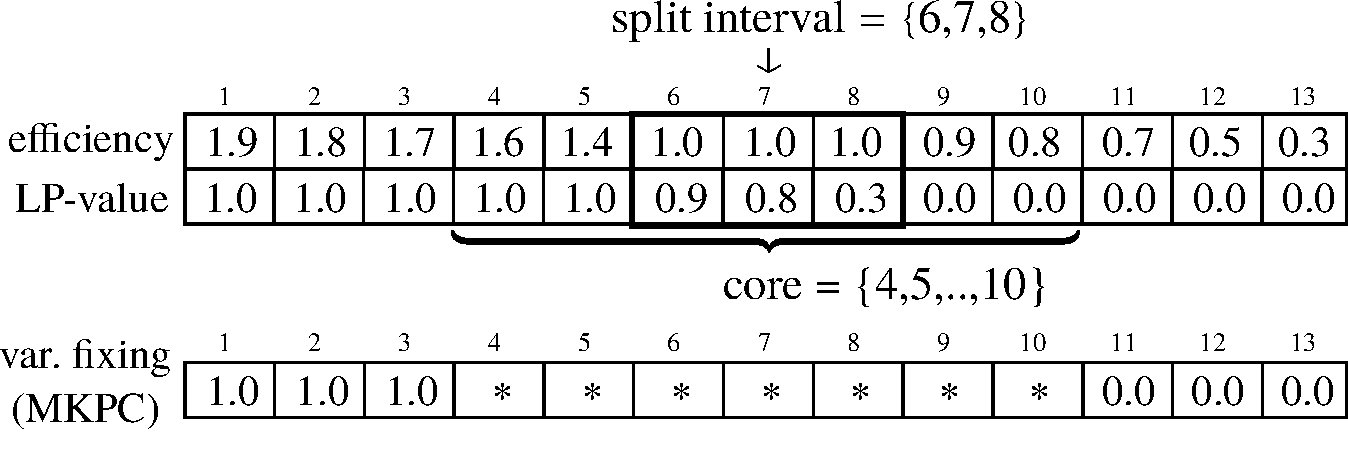
\includegraphics[scale=0.37]{imgs/mkp_2}
  \caption{Example of core for a hypothetical MKP instace with $n=13$, $m=3$ and core size of $7$ ($\delta = 3$).}
  \label{fig:mkpcore}
\end{figure}


\cite{puchinger2006core}

% - Eficieny measure...
% - the core problem (KPC)
% - core concept for MKP
%  - Efficiency measure... (sketch...) the dual efficieny measure
%  - the Multidimentional kanspack core problem (MKPC)

